\documentclass[journal]{IEEEtran}
\usepackage{cite}
\usepackage{amsmath,amssymb}
\usepackage{graphicx}
\usepackage{booktabs}
\usepackage{multirow}
\usepackage{algorithm}
\usepackage{algpseudocode}
\algrenewcommand\algorithmicrequire{\textbf{Input:}}
\algrenewcommand\algorithmicensure{\textbf{Output:}}
\usepackage{tikz}
\usetikzlibrary{positioning,arrows.meta,fit}
\usepackage[hidelinks]{hyperref}

\newcommand{\Exp}{\operatorname{Exp}}
\newcommand{\Log}{\operatorname{Log}}
\newcommand{\tr}{\operatorname{tr}}

\begin{document}

\title{CSD-LVIO: Channel-Separated, Consistency-Gated\\ LiDAR-Visual-Inertial Odometry for Degenerate Environments}

\author{Kavinkumar~S and G.~Sivasankar%
\thanks{The authors are with Amrita School of Engineering, Coimbatore, Amrita Vishwa Vidyapeetham, India.}}

\markboth{Preprint, November 2026}{Kavinkumar and Sivasankar: CSD-LVIO}

\maketitle

\begin{abstract}
LiDAR odometry loses accuracy along directions that the scene does not constrain, such as the axis of a corridor, while visual-inertial odometry (VIO) fails under fast rotation, darkness and poor initialisation. Switching-based systems pick one source when the other is judged degenerate, but a binary decision on the whole pose discards the LiDAR information that remains in the constrained directions. We present CSD-LVIO, a loosely coupled front end that fuses A-LOAM and VINS-Mono per scan and per direction. The registration Hessian is split by Schur complements into a rotation channel and a translation channel. The translation channel sets an information weight along each eigen-direction, and an orientation tensor computed from the raw scan geometry adds support that the solver under-reports. The VIO is trusted only while its scale agrees with the LiDAR, a guard catches LiDAR blow-ups, and the hand-over between modes is anchored to avoid heading steps. A degeneracy-gated prediction takes the scan-to-map initial guess from the LiDAR unless the scan is degenerate. All constants were fixed on one calibration sequence. On the SubT-MRS Multi Floor and Long Corridor sequences the front end reaches 0.54 m and 2.10 m ATE RMSE against 1.61 m and 2.42 m published for Switch-SLAM. On Corridor02, where A-LOAM alone diverged in every run, it reaches 1.99 m, and on Cave02 and the GEODE stairs it leaves 5 to 6 m. We report every run, including one divergence of the variant without gated prediction, and discuss how far the small number of runs and the shared development data limit these comparisons.
\end{abstract}

\begin{IEEEkeywords}
LiDAR degeneracy, sensor fusion, visual-inertial odometry, SLAM, Schur complement.
\end{IEEEkeywords}

\section{Introduction}
\IEEEPARstart{L}{iDAR} odometry and mapping \cite{loam2014,liosam2020,fastlio2} is accurate where the geometry constrains all six degrees of freedom, and it degrades where it does not. In a long corridor the translation along the axis is unobservable; on a staircase or in a cave the constraint is weak and changes from scan to scan. Visual-inertial odometry \cite{vinsmono2018} has the opposite profile. It keeps its scale in featureless corridors as long as the camera tracks texture, and it drifts or re-initialises under darkness, fast rotation or a poor start \cite{cadena2016,ebadi2024}.

Tightly coupled LiDAR-visual-inertial systems \cite{lvisam2021,r2live2021,r3live2022,fastlivo2022,superodom2021} fuse both sources in one maximum a posteriori estimate. Lee \emph{et al.} \cite{switchslam2024} argue that such fusion lets a long failure of one sensor corrupt the whole estimate, and propose Switch-SLAM, which selects the scan-to-map initial guess from LiDAR or VIO with a parameter-free eigenvalue test and remaps the solution along the degenerate directions. A test on the whole Hessian makes one decision for all six directions. In a corridor, the LiDAR still fixes the two lateral translations and all three rotations, and a switch spends that information.

This letter describes a front end that keeps both odometries running and fuses them per direction. Our contributions are:
\begin{enumerate}
\item A channel-separated weighting. Schur complements of the registration Hessian give a rotation block and a translation block in their own units. The translation block sets a per-direction information weight between the LiDAR and VIO increments, and an orientation tensor of the raw scan geometry supplies support that the solver under-reports.
\item A consistency-gated trust of the VIO. A scale-consistency gate, a rotation-consistency check, a LiDAR blow-up guard and an anchored hand-over decide when each source may carry a step. Their constants come from one calibration sequence and were not refitted.
\item A degeneracy-gated prediction that uses the switching rule of \cite{switchslam2024} only for the scan-to-map initial guess, while the output stays the fused estimate.
\item A live evaluation on five real sequences with ground truth, against the published Switch-SLAM results and against our own re-implementation of it in the same pipeline, with every run reported and a one-sided significance test for each comparison.
\end{enumerate}

\section{Related Work}
\subsection{Detecting and handling LiDAR degeneracy}
Gelfand \emph{et al.} \cite{gelfand2003} related ICP stability to the eigenvalues of the point-to-plane information matrix. Zhang \emph{et al.} \cite{zhang2016} thresholded the eigenvalues of the registration Hessian and updated the solution only in the well-conditioned directions (solution remapping), and Hinduja \emph{et al.} \cite{hinduja2019} carried the same idea into degeneracy-aware factors for pose graphs. Later work replaced the fixed threshold by a localizability analysis of the correspondences (X-ICP \cite{xicp2024}, LP-ICP \cite{lpicp2025}), a learned predictor \cite{nubert2022}, or a probabilistic test \cite{hatleskog2024}. Tuna \emph{et al.} \cite{tuna2025} compared these strategies in the field and found that mitigation matters most when no reliable external prior exists. DCReg \cite{dcreg2026} decouples the Hessian into rotation and translation subspaces with Schur complements before characterising ill-conditioning, the same decomposition we use, but it acts inside the registration solver, while we use it to weight two odometries. NV-LIOM \cite{nvliom2024} uses normal vectors from range images to detect degeneracy in multi-floor buildings.

\subsection{Combining LiDAR and visual-inertial odometry}
LVI-SAM \cite{lvisam2021} seeds scan matching with VIO, which makes it sensitive to VIO failures \cite{switchslam2024}. R$^2$LIVE \cite{r2live2021}, R$^3$LIVE \cite{r3live2022} and FAST-LIVO \cite{fastlivo2022} fuse all measurements in an iterated Kalman filter, and Super Odometry \cite{superodom2021} centres the estimate on the IMU. RELEAD \cite{relead2024} adds degeneracy-aware constraints to LiDAR odometry. Switch-SLAM \cite{switchslam2024} is the closest to our setting. It runs both odometries in parallel, chooses the initial guess by a chi-squared bound on the three smallest normalised Hessian eigenvalues, interpolates over a status buffer at the start and end of a degenerate stretch, and remaps the solution. Our system differs in that the output is never switched as a whole: every scan is a per-direction weighted combination, and the switching rule only decides the initial guess.

\section{Method}
\subsection{Overview and notation}
Fig.~\ref{fig:overview} shows the structure. A-LOAM \cite{aloam} provides, for every scan $k$, its scan-to-map pose $(\mathbf R_{A,k},\mathbf p_{A,k})$ and the $6\times6$ Hessian $\mathbf H$ of its scan-to-scan registration. VINS-Mono \cite{vinsmono2018} runs unchanged and provides an IMU pose, moved into the LiDAR frame with the extrinsic calibration. From consecutive poses we form the increments $(\Delta\mathbf R_L,\Delta\mathbf t_L)$ of the LiDAR and $(\Delta\mathbf R_V,\Delta\mathbf t_V)$ of the VIO, both in the body frame of scan $k-1$. The fused pose is propagated as
\begin{align}
\Delta\mathbf t &= \mathbf W_t\,\Delta\mathbf t_L + (\mathbf I-\mathbf W_t)\,\Delta\mathbf t_V, \label{eq:t}\\
\boldsymbol\phi &= \mathbf W_R\,\Log(\Delta\mathbf R_L) + (\mathbf I-\mathbf W_R)\,\Log(\Delta\mathbf R_V), \label{eq:r}
\end{align}
with $\mathbf R_k=\mathbf R_{k-1}\Exp(\boldsymbol\phi)$ and $\mathbf p_k=\mathbf p_{k-1}+\mathbf R_{k-1}\Delta\mathbf t$. The weights $\mathbf W_t,\mathbf W_R$ are $3\times3$ matrices, so each direction has its own balance. Algorithm~\ref{alg:node} lists the whole per-scan procedure. The node has four modes: a warm-up of 20\,s after VIO (re)starts and a failure mode, in both of which the LiDAR carries the step ($\mathbf W_t=\mathbf W_R=\mathbf I$); the fused mode; and an initial mode.

\begin{figure}[t]
\centering
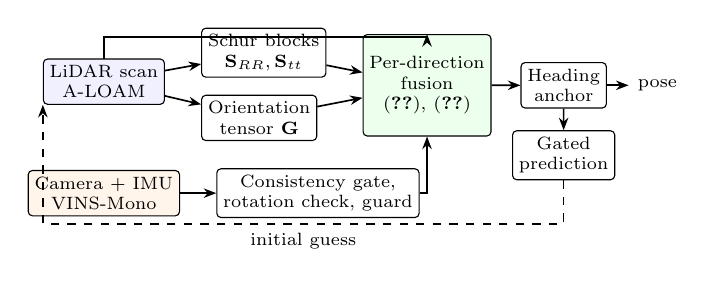
\begin{tikzpicture}[font=\scriptsize, scale=0.92, transform shape, node distance=3.5mm and 4mm,
  box/.style={draw, rounded corners=1.5pt, align=center, inner sep=2.5pt, minimum height=6mm},
  arr/.style={-{Stealth[length=1.6mm]}, semithick}]
\node[box, fill=blue!6] (lidar) {LiDAR scan\\A-LOAM};
\node[box, fill=orange!8, below=9mm of lidar] (vio) {Camera + IMU\\VINS-Mono};
\node[box, right=5mm of lidar, yshift=4mm] (schur) {Schur blocks\\$\mathbf S_{RR},\mathbf S_{tt}$};
\node[box, right=5mm of lidar, yshift=-5mm] (ot) {Orientation\\tensor $\mathbf G$};
\node[box, right=5mm of vio] (gate) {Consistency gate,\\rotation check, guard};
\node[box, fill=green!7, right=5mm of schur, yshift=-4.5mm, minimum height=14mm] (fuse) {Per-direction\\fusion\\(\ref{eq:t}), (\ref{eq:r})};
\node[box, right=4mm of fuse] (sah) {Heading\\anchor};
\node[box, below=3mm of sah] (dgp) {Gated\\prediction};
\draw[arr] (lidar) -- (schur); \draw[arr] (lidar) -- (ot);
\draw[arr] (schur) -- (fuse); \draw[arr] (ot) -- (fuse);
\draw[arr] (vio) -- (gate); \draw[arr] (gate) -| (fuse);
\draw[arr] (lidar.north) |- ++(0,3mm) -| (fuse.north);
\draw[arr] (fuse) -- (sah);
\draw[arr] (sah.east) -- ++(3mm,0) node[right, align=left]{pose};
\draw[arr] (sah) -- (dgp);
\draw[arr, dashed] (dgp.south) |- ++(0,-6mm) -| node[pos=0.25, below]{initial guess} (lidar.south west);
\end{tikzpicture}
\caption{Structure of CSD-LVIO. Both odometries run unchanged. The fusion node weights their increments per direction, gates the VIO by consistency, anchors heading to wall structure and returns a degeneracy-gated initial guess to the scan-to-map matching.}
\label{fig:overview}
\end{figure}

\subsection{Rotation and translation channels}
Let $\mathbf H$ be expressed in radians and metres and split into $3\times3$ blocks. The Schur complements
\begin{equation}
\mathbf S_{tt}=\mathbf H_{tt}-\mathbf H_{tR}\mathbf H_{RR}^{-1}\mathbf H_{Rt},\qquad
\mathbf S_{RR}=\mathbf H_{RR}-\mathbf H_{Rt}\mathbf H_{tt}^{-1}\mathbf H_{tR}
\end{equation}
are the translation information left once rotation is free, and the reverse. Each block has one unit, so its eigenvalues can be compared, which is not true of the full Hessian, where rotational and translational eigenvalues mix units. In a corridor $\mathbf S_{tt}$ has one small eigenvalue along the axis and two large ones across it.

The translation channel treats the LiDAR increment as a measurement with information $c_T\mathbf S_{tt}$ and the VIO increment as a prior with information $\gamma\mathbf I$:
\begin{equation}
\mathbf W_t=(c_T\mathbf S'_{tt}+\gamma\mathbf I)^{-1}c_T\mathbf S'_{tt}, \label{eq:wt}
\end{equation}
where $\mathbf S'_{tt}$ is $\mathbf S_{tt}$ after the support check of Section~\ref{sec:ot}. Along an eigenvector with eigenvalue $\lambda$ the weight is $c_T\lambda/(c_T\lambda+\gamma)$. It is close to one where the scene constrains the motion and close to zero along a degenerate axis, with no switching threshold. The scale $c_T=0.03$ was chosen once on Multi Floor. The gate value $\gamma$ is described in Section~\ref{sec:gate}.

With A-LOAM, the VINS-Mono rotation was better than the LiDAR rotation on most sequences in replay, so in the fused mode $\mathbf W_R=\mathbf 0$ and $\mathbf S_{RR}$ is monitored. A rotation-consistency check accumulates $\|\Log(\Delta\mathbf R_L^{\top}\Delta\mathbf R_V)\|$ over 2\,s and 10\,s windows. If it exceeds 0.402\,rad or 0.585\,rad, the largest values seen on 19 Multi Floor recordings, the LiDAR rotation carries the step with $\mathbf W_R=(\mathbf S_{RR}+10^{-3}\mathbf I)^{-1}\mathbf S_{RR}$.

\subsection{Orientation-tensor support}\label{sec:ot}
The Hessian reflects only the correspondences that A-LOAM accepted in one scan. As a second opinion that uses no correspondence, at every keyframe (1\,m or 0.2\,rad of motion) we classify each point by the eigenvalues $\mu_1\le\mu_2\le\mu_3$ of its 12-neighbour covariance as planar, with normal $\mathbf n$, when $(\mu_2-\mu_1)/\mu_3>0.5$, or linear, with direction $\mathbf d$, when $(\mu_3-\mu_2)/\mu_3>0.5$, and form
\begin{equation}
\mathbf G=\frac{1}{n_p+n_l}\Big(\sum_{\text{planar}}\mathbf n\mathbf n^{\top}+\tfrac12\sum_{\text{linear}}(\mathbf I-\mathbf d\mathbf d^{\top})\Big).
\end{equation}
A plane constrains translation along its normal and an edge in the plane perpendicular to it. $\mathbf G$ has unit trace and uses no correspondence and no solver state. It is scaled to the solver's total information, $\mathbf B=\tr(\mathbf H_{tt})\,\mathbf G$, rotated into the current frame, and combined with $\mathbf A=\mathbf S_{tt}$ by the generalised maximum
\begin{equation}
\mathbf S'_{tt}=\mathbf B^{1/2}\max(\mathbf M,\mathbf I)\,\mathbf B^{1/2},\qquad \mathbf M=\mathbf B^{-1/2}\mathbf A\mathbf B^{-1/2},
\end{equation}
which raises every generalised eigenvalue below one to one, so along each direction the larger of the two supports is kept. This rule is optimistic; the protection against a solver that is confident and wrong comes from the gate below. A tensor of planar normals alone understated the support from door frames and pipes and made the corridor sequences 0.26 to 1.0\,m worse in replay.

\subsection{Consistency gate and guards}\label{sec:gate}
Within one VIO segment, every scan closes a 10\,s window. For windows with at least 1\,m of LiDAR motion we form $x=\ln(\|\Delta\mathbf p_V\|/\|\Delta\mathbf p_L\|)$, and $r=\sqrt{\overline{x^2}}$ over the segment and over the windows that ended in the last 5\,s. The VIO is trusted, $\gamma=1$ in (\ref{eq:wt}), while $r\le0.157$ and the fast value is $\le0.277$; otherwise $\gamma=0$ and $\mathbf W_t=\mathbf I$. The VIO is trusted at the start of a segment until enough windows exist (200 for the segment test, 25 for the fast one).

Three guards act on single steps. A VIO step above 1\,m or 0.5\,rad marks a VIO failure and restarts the warm-up. While the VIO is trusted, a LiDAR path that runs more than 4.325\,m ahead of the VIO path within 2\,s marks the LiDAR step as failed, and the VIO carries it. At every entry into the fused mode the orientation is reset to
\begin{equation}
\mathbf R_f=\mathbf R_{\text{off}}\,\mathbf R_{VL},\qquad \mathbf R_{\text{off}}=\operatorname{mean}_j\big(\mathbf R_{A,j}\mathbf R_{VL,j}^{\top}\big),
\end{equation}
where $\mathbf R_{VL}$ is the LiDAR orientation predicted by the VIO and the robust chordal mean runs over the warm-up scans. Without this anchor the fused heading jumped by 6 to 7$^\circ$ at the first fused scan of Long Corridor, because the warm-up had already integrated a fast turn that the lagging VIO then added again.

\subsection{Structure-anchored heading}
Heading is unobservable for the VIO and dominates the error in long corridors. At each keyframe the near-vertical planar normals are levelled with the VIO gravity direction, and their horizontal directions form an axial histogram $h(\theta)$ with 0.5$^\circ$ bins over 180$^\circ$. The heading error is the shift, searched over $\pm15^\circ$, that best aligns $h$ with a reference histogram learned in the world frame. It passes a Kalman update and is applied at no more than 0.25$^\circ$ per scan. It switches itself off when the structure is not distinct, using a test against random directions, a unique correlation peak, a chi-squared gate and a drift gate.

\subsection{Degeneracy-gated prediction}
A-LOAM starts each scan-to-map registration from a predicted pose. We compose the last fused pose with an increment $\boldsymbol\delta$ chosen by the rule of \cite{switchslam2024}: the three smallest eigenvalues of $\mathbf H$ are normalised to unit norm, $\bar{\boldsymbol\lambda}$, and the scan is degenerate if any $\bar\lambda_i$ lies below $[0.12,\,0.27,\,0.48]_i$. A status queue of the last five scans gives
\begin{equation}
\boldsymbol\delta=\begin{cases}
\boldsymbol\delta_L & \text{(a)},\\
\sqrt3\bar\lambda_1\boldsymbol\delta_L\oplus(1-\sqrt3\bar\lambda_1)\boldsymbol\delta_V & \text{(b)},\\
\boldsymbol\delta_V & \text{(c)},
\end{cases}
\end{equation}
where case (a) holds when the scan is not degenerate or the VIO is unusable, (b) when the queue holds both states and (c) when it holds only degenerate scans. Here $\boldsymbol\delta_L$ is A-LOAM's scan-to-scan increment, $\boldsymbol\delta_V$ the VIO increment, and $\oplus$ combines increments in the tangent space. The VIO is unusable after a failure step or for a step above the 1\,m or 0.5\,rad limits. Without this rule, the system used the VIO increment whenever it was usable and no motion otherwise; Section~\ref{sec:ablation} compares the two.

\subsection{Per-scan procedure}
Algorithm~\ref{alg:node} puts the parts together for one scan. Lines 1 to 20 form the fusion of Sections III-B to III-E, and lines 21 to 30 the gated prediction of Section III-F, which returns A-LOAM's initial guess; the source of every constant is given in Table~\ref{tab:const}.

\begin{algorithm}[t]
\caption{Fusion node with degeneracy-gated prediction}\label{alg:node}
\footnotesize
\begin{algorithmic}[1]
\Require previous pose $\mathbf T_{k-1}$; A-LOAM Hessian $\mathbf H$ and increment $\boldsymbol\delta_L$; VIO increment $\boldsymbol\delta_V$ and status $S_{vo}$; orientation tensor $\mathbf G$; status queue $Q_s$ of size 5; mode
\Ensure fused pose $\mathbf T_k$; initial guess $\mathbf T^{\mathrm{init}}_{k+1}$ for A-LOAM
\State $u\leftarrow (S_{vo}=\text{fail})\ \vee\ \|\boldsymbol\delta_V\|$ above 1\,m or 0.5\,rad \Comment{VIO unusable}
\If{$u$} mode $\leftarrow$ failure; restart the 20\,s warm-up \EndIf
\If{mode $\in\{$warm-up, failure$\}$}
  \State $\mathbf W_t\leftarrow\mathbf I,\ \mathbf W_R\leftarrow\mathbf I$ \Comment{the LiDAR carries the step}
\Else
  \If{first fused scan of the segment}
    \State $\mathbf R_{k-1}\leftarrow\mathbf R_{\mathrm{off}}\mathbf R_{VL}$ \Comment{anchored hand-over}
  \EndIf
  \State $\mathbf S_{tt},\mathbf S_{RR}\leftarrow$ Schur complements of $\mathbf H$
  \State $\mathbf S'_{tt}\leftarrow$ generalised maximum of $\mathbf S_{tt}$ and $\mathrm{tr}(\mathbf H_{tt})\mathbf G$ \Comment{tensor}
  \State update $r$ and $r_{\mathrm{fast}}$; $\gamma\leftarrow 1$ if $r\le0.157$ and $r_{\mathrm{fast}}\le0.277$, else $0$
  \State $\mathbf W_t\leftarrow(c_T\mathbf S'_{tt}+\gamma\mathbf I)^{-1}c_T\mathbf S'_{tt}$ \Comment{translation channel}
  \State $\mathbf W_R\leftarrow\mathbf 0$; \textbf{if} rotation check above 0.402\,rad (2\,s) or 0.585\,rad (10\,s) \textbf{then} $\mathbf W_R\leftarrow(\mathbf S_{RR}+10^{-3}\mathbf I)^{-1}\mathbf S_{RR}$
  \If{LiDAR path leads the VIO path by more than 4.325\,m within 2\,s}
    \State $\mathbf W_t\leftarrow\mathbf 0$ \Comment{LiDAR step failed, the VIO carries it}
  \EndIf
\EndIf
\State $\Delta\mathbf t\leftarrow\mathbf W_t\Delta\mathbf t_L+(\mathbf I-\mathbf W_t)\Delta\mathbf t_V$;\ $\boldsymbol\phi\leftarrow\mathbf W_R\mathrm{Log}(\Delta\mathbf R_L)+(\mathbf I-\mathbf W_R)\mathrm{Log}(\Delta\mathbf R_V)$
\State $\mathbf T_k\leftarrow\mathbf T_{k-1}\oplus(\boldsymbol\phi,\Delta\mathbf t)$; apply the heading correction, at most $0.25^\circ$ per scan
\State $\bar{\boldsymbol\lambda}\leftarrow$ three smallest eigenvalues of $\mathbf H$, normalised; flag $\leftarrow\exists i:\bar\lambda_i<\lambda_{t,i}$, with $\boldsymbol\lambda_t=[0.12,0.27,0.48]$
\If{$u$ or no scan in $Q_s$ is degenerate}
  \State $\boldsymbol\delta\leftarrow\boldsymbol\delta_L$ \Comment{A-LOAM's own increment}
\ElsIf{$Q_s$ holds both states}
  \State $\boldsymbol\delta\leftarrow\sqrt3\bar\lambda_1\boldsymbol\delta_L\oplus(1-\sqrt3\bar\lambda_1)\boldsymbol\delta_V$ \Comment{interpolation}
\Else
  \State $\boldsymbol\delta\leftarrow\boldsymbol\delta_V$ \Comment{only degenerate scans}
\EndIf
\State $\mathbf T^{\mathrm{init}}_{k+1}\leftarrow\mathbf T_k\oplus\boldsymbol\delta$; dequeue $Q_s$ and enqueue flag
\State \Return $\mathbf T_k,\ \mathbf T^{\mathrm{init}}_{k+1}$
\end{algorithmic}
\end{algorithm}

\begin{table}[t]
\caption{Frozen constants}
\label{tab:const}
\centering\footnotesize
\resizebox{\columnwidth}{!}{%
\begin{tabular}{@{}lll@{}}
\toprule
Constant & Value & Source\\\midrule
$c_T$ (translation scale) & 0.03 & Multi Floor, once\\
$c_R$ in fused mode & 0 & Replay (VIO rotation better)\\
Warm-up & 20\,s & Design value\\
VIO step limits & 1\,m, 0.5\,rad & Design value\\
Rotation check & 0.402 rad / 2\,s, 0.585 rad / 10\,s & 19 Multi Floor recordings\\
Scale gate & 0.157 (segment), 0.277 (5\,s) & 6 Multi Floor replays\\
LiDAR guard & 4.325\,m over 2\,s & 6 Multi Floor replays\\
Tensor $k$-NN, shape cut & 12, 0.5 & Shared with heading\\
Heading search, step & $\pm15^\circ$, $0.25^\circ$/scan & Long Corridor, Corridor02\\
Prediction thresholds & $[0.12, 0.27, 0.48]$, queue 5 & From \cite{switchslam2024}\\
\bottomrule
\end{tabular}}
\end{table}

\section{Experimental Setup}
\subsection{Sequences}
Table~\ref{tab:seq} lists the five real sequences. Multi Floor and Long Corridor are the two SubT-MRS \cite{subtmrs2024} sequences on which Switch-SLAM reports results \cite{switchslam2024}. Corridor02 and Cave02, also from SubT-MRS, add a longer corridor and a dark cave. GEODE stairs alpha \cite{geode2026} is a staircase from a dataset built around degenerate scenes. All have ground-truth trajectories.

\begin{table}[t]
\caption{Sequences}
\label{tab:seq}
\centering\footnotesize
\resizebox{\columnwidth}{!}{%
\begin{tabular}{@{}lrrll@{}}
\toprule
Sequence & Path (m) & Time (s) & Main difficulty & Replay\\\midrule
Multi Floor & 272.7 & 417 & Stairwells between floors & 1.0$\times$\\
Long Corridor & 579.2 & 279 & Long uniform corridor & 0.5$\times$\\
Corridor02 & 695.2 & 893 & Long corridors, loops & 0.33$\times$\\
Cave02 & 475.0 & 954 & Dark, irregular cave & 0.5$\times$\\
GEODE stairs & 301.1 & 345 & Staircase, weak structure & 0.5$\times$\\
\bottomrule
\end{tabular}}
\end{table}

\subsection{Implementation and metric}
A-LOAM \cite{aloam} is patched to publish the Hessian of its scan-to-scan registration, and its mapping stage takes the predicted pose from the fusion node in place of its own odometry. VINS-Mono runs unchanged in its own container. The fusion node is written in Python. All runs are live: the bag is replayed through the whole pipeline on one laptop (AMD Ryzen 5 5600H), at the rates in Table~\ref{tab:seq}, because the pipeline does not keep up at full rate on longer sequences. The metric is the absolute trajectory error of the front end without loop closure: the estimated positions are aligned to the ground truth by the rigid transformation without scale \cite{umeyama1991} over the full span, and we report the RMSE and the maximum, as \cite{switchslam2024} does.

\subsection{Protocol}
The constants in Table~\ref{tab:const} were fixed on Multi Floor and not changed afterwards. Multi Floor is therefore calibration data, and Long Corridor and Corridor02 were used while designing the heading anchor and the guards. Cave02 and GEODE were first run after the configuration without gated prediction was frozen, but the gated prediction was added after those runs, so for the final system no sequence is strictly held out. The prediction rule adds no fitted constant; its thresholds are those of \cite{switchslam2024}. Every completed run is reported, failures included.

\emph{Significance tests.} Following the format of Ganesan \emph{et al.} \cite{ganesan2024}, each comparison tests $H_0$: the median ATE RMSE of the baseline equals that of CSD-LVIO, against $H_1$: the baseline is larger, at the 5\,\% level. We use the exact one-sided Mann-Whitney test, whose null distribution is enumerated over all arrangements of the pooled runs, so that no normal approximation is needed with so few runs, and add Welch's $t$-test where both groups have at least two runs. With $n$ baseline runs and $m$ runs of CSD-LVIO the smallest possible $p$ is $1/\binom{n+m}{m}$, so one CSD-LVIO run against three baseline runs cannot go below 0.25. The Farm has one run per method and is not tested. The published Switch-SLAM values are single numbers and cannot be tested.

\subsection{Baselines}
We report A-LOAM alone and VINS-Mono alone in our pipeline, the published Switch-SLAM results \cite{switchslam2024} (mean of three runs, real time on an Intel i7-1165G7), and our re-implementation of Switch-SLAM. No code of Switch-SLAM has been released. Our re-implementation follows its Algorithm 1 and Eqs. (11) to (16) on the same A-LOAM and VINS-Mono, but A-LOAM's scan-to-scan increment replaces the IMU-propagated LiDAR odometry of the original, and the remap is applied to A-LOAM's converged solution instead of inside the solver.

\section{Results}
\begin{table*}[t]
\caption{ATE of the front end, RMSE / max in metres; $n$ = number of live runs, mean over runs. ``--'': not available.}
\label{tab:main}
\centering\footnotesize
\resizebox{\textwidth}{!}{%
\begin{tabular}{@{}lccccc@{}}
\toprule
Method & Multi Floor & Long Corridor & Corridor02 & Cave02 & GEODE stairs\\\midrule
A-LOAM \cite{aloam}, our pipeline & 26.4 / --$^{c}$ ($n$=3) & 15.8 / --$^{c}$ ($n$=3) & 46.5 to 93.0 ($n$=4, all diverged) & -- & 7.98 / 22.09 ($n$=1)\\
VINS-Mono \cite{vinsmono2018}, our configuration & 1.32 / 4.77 ($n$=4) & 5.15 / 11.39 ($n$=4) & 3.52 / 8.38 ($n$=5) & 10.8 to 34.1$^{a}$ ($n$=4) & 153 to 272$^{a}$ ($n$=7)\\
Switch-SLAM, published \cite{switchslam2024} & 1.61 / 3.63 & 2.42 / 5.09 & -- & -- & --\\
Switch-SLAM, our re-implementation & 5.24 / 10.58 ($n$=2) & 12.85 / 23.50 ($n$=2) & -- & -- & --\\\midrule
CSD-LVIO without gated prediction & 0.72 / 1.30 ($n$=3) & \textbf{2.01} / 4.80 ($n$=3) & \textbf{1.38} / \textbf{2.60}$^{b}$ ($n$=3) & 7.25 / 12.06 ($n$=3) & 7.23 / 18.25 ($n$=4)\\
CSD-LVIO & \textbf{0.54} / \textbf{1.01} ($n$=1) & 2.10 / \textbf{3.73} ($n$=1) & 1.99 / 3.46 ($n$=2) & \textbf{6.23} / \textbf{10.56} ($n$=1) & \textbf{5.04} / \textbf{12.38} ($n$=3)\\
\bottomrule
\end{tabular}}\\[2pt]
\raggedright\scriptsize $^{a}$ VINS-Mono had failure steps in every run (11 to 175 on Cave02, 871 to 1282 on GEODE); range of RMSE over the runs. VINS-Mono runs independently of the fusion, so its rows are read from the logs of the fused runs. $^{b}$ Mean of the two runs that completed normally; the third run diverged at 104.00 / 149.20 m (Section~\ref{sec:ablation}). $^{c}$ Earlier batch at 1.0$\times$ replay; maximum not recorded.
\end{table*}

\subsection{Accuracy against the baselines}
Table~\ref{tab:main} gives the results. On Multi Floor CSD-LVIO reached 0.54\,m RMSE and 1.01\,m maximum, against 1.61 / 3.63\,m published for Switch-SLAM. On Long Corridor it reached 2.10 / 3.73\,m against 2.42 / 5.09\,m. The variant without gated prediction gave 0.72 / 1.30\,m and 2.01 / 4.80\,m over three runs each, with run-to-run ranges of 0.45 to 1.01\,m and 1.75 to 2.15\,m, so the comparison with the published numbers does not depend on one favourable run of one variant.

Two facts limit this comparison. First, our VINS-Mono configuration alone reaches 1.32\,m on Multi Floor and 5.15\,m on Long Corridor, where the Switch-SLAM letter reports 6.30\,m and 11.8\,m for VINS-Mono; part of the gap therefore lies in the front ends, not in the fusion. Second, our re-implementation of Switch-SLAM in the same pipeline gave 5.24\,m and 12.85\,m, far from the published values. With its rule the scan was degenerate on only 1.5\,\% of Multi Floor scans and 4.5\,\% of Long Corridor scans, so it behaved mostly like A-LOAM, whose guess in our pipeline lacks the IMU propagation of the original. We therefore read the re-implementation as a lower bound on Switch-SLAM in our pipeline, not as a reproduction.

Relative to the two single sources, the fusion was below both on Multi Floor (VINS-Mono 1.32\,m, A-LOAM 26.4\,m), Long Corridor (5.15\,m and 15.8\,m) and Corridor02, where A-LOAM alone diverged in all four runs and VINS-Mono reached 3.52\,m. On Corridor02 the fused trajectory follows the ground truth over 695\,m (Fig.~\ref{fig:traj}).

\begin{figure}[t]
\centering
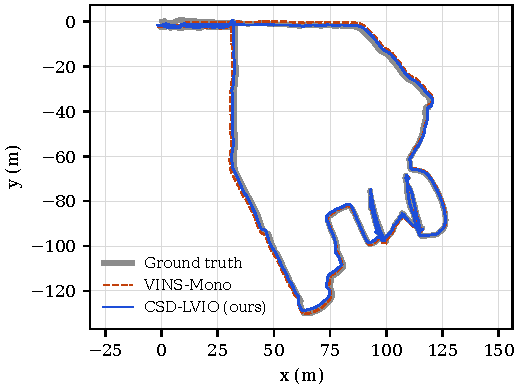
\includegraphics[width=\columnwidth]{figures/corridor02_topview.pdf}
\caption{Corridor02, top view after rigid alignment: ground truth, VINS-Mono alone and CSD-LVIO (run 1, 1.93\,m RMSE).}
\label{fig:traj}
\end{figure}

\subsection{Effect of the gated prediction}\label{sec:ablation}
Fig.~\ref{fig:runs} shows every run of both variants. With gated prediction the mean RMSE was lower on Multi Floor (0.54 against 0.72\,m), Cave02 (6.23 against 7.25\,m) and GEODE (5.04 against 7.23\,m), about the same on Long Corridor (2.10 against 2.01\,m), and higher on the two normal Corridor02 runs (1.99 against 1.38\,m). On GEODE the three runs with gated prediction (3.26 to 6.36\,m) and the four without (6.15 to 9.15\,m) barely overlap. An exact Mann-Whitney test gives $U=1$, one-sided $p=0.057$, which is suggestive and not significant.

The mechanism is visible in the logs. Without gated prediction, the predicted pose carried no motion whenever the VIO was unusable, which happened on 13.5\,\% of Cave02 scans (the first 130\,s, where 14 to 36\,\% of the squared error arises) and on 78\,\% of GEODE scans. A-LOAM then started each registration one scan behind. With the gated rule, A-LOAM's own increment is used in that case, and since the eigenvalue test fires on few scans (0.0\,\% of Cave02, 10.3\,\% of GEODE), the guess came from the LiDAR on 100\,\% and 93.7\,\% of scans. Comparing the first run of each variant on Cave02 (Fig.~\ref{fig:cave}), the error with gated prediction was lower in every 120\,s block, from 12.0 to 9.7\,m in the first block and from 4.9 to 5.8\,m down to 4.1 to 5.0\,m in the later ones.

\begin{figure}[t]
\centering
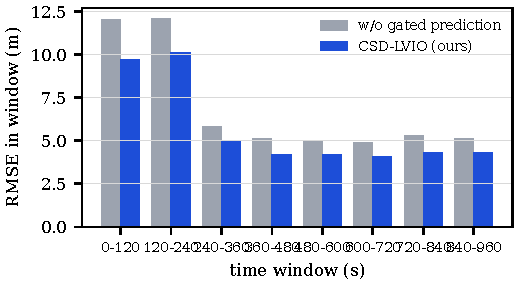
\includegraphics[width=\columnwidth]{figures/cave02_blocks.pdf}
\caption{Cave02, first run of each variant: RMSE per 120\,s window. The gated prediction lowers every window; the first 240\,s dominate both runs.}
\label{fig:cave}
\end{figure}

One run of the variant without gated prediction diverged on Corridor02 (104.00\,m). The logs show that A-LOAM turned the wrong way at about 545\,s: its trajectory and the VIO's separated from 6\,m to 49\,m within 7\,s. The rotation check closed for about 10\,s, which hands the rotation to the LiDAR, the scale gate closed for a single scan, and the fused pose followed A-LOAM. VINS-Mono alone was normal in that run (3.55\,m). The two runs with gated prediction on Corridor02 did not diverge; two runs cannot establish a failure rate, so we report this as an observed failure mode of the system, not as an effect of the prediction.

\begin{figure}[t]
\centering
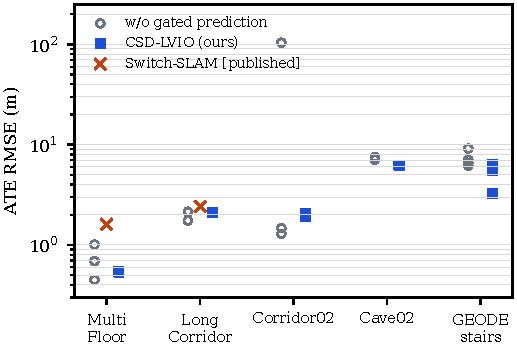
\includegraphics[width=\columnwidth]{figures/per_run_rmse.pdf}
\caption{ATE RMSE of every live run, logarithmic scale. The diverged Corridor02 run of the variant without gated prediction is the point at 104\,m.}
\label{fig:runs}
\end{figure}

\subsection{Hypothesis tests}\label{sec:hyp}
Table~\ref{tab:hyp} gives the tests of Section~IV-C for every baseline that has runs on the same sequence. CSD-LVIO was lower than the baseline in every pairing of runs against VINS-Mono alone and A-LOAM alone. Only the GEODE comparison with VINS-Mono alone rejects $H_0$ with the exact test ($p=0.008$, 21 of 21 pairs; Welch $p=1.7\times10^{-5}$). On Corridor02 the exact test cannot go below 0.10 with three and two runs, and Welch's test rejects against VINS-Mono alone ($p=0.008$) and A-LOAM alone ($p=0.022$). On Multi Floor, Long Corridor and Cave02 one run of CSD-LVIO sets the limit at $p=0.25$, so the test cannot reject whatever the numbers are.

Against the variant without gated prediction no test rejects. On GEODE CSD-LVIO was lower in 11 of 12 pairs ($p=0.057$, Welch $p=0.065$, and $p=0.114$ for the maximum error), and on Corridor02 it was higher in four of six pairs, those against the two normal runs of the variant (the diverged run of 104\,m accounts for the other two). The tests therefore support one claim, that the fusion is reliably better than VINS-Mono alone where VINS-Mono fails, and none about the gated prediction, which the data show only as a lower mean on three sequences.

\begin{table}[t]
\caption{One-sided tests of $H_0$: median ATE RMSE of the baseline equals that of CSD-LVIO, against $H_1$: baseline larger. $n$: runs of the baseline / of CSD-LVIO. Exact Mann-Whitney $p$ for the RMSE and the maximum error, Welch $p$ for the RMSE. ``--'': not computed (one run in a group, or maximum not recorded).}
\label{tab:hyp}
\centering\scriptsize
\setlength{\tabcolsep}{3pt}
\resizebox{\columnwidth}{!}{%
\begin{tabular}{@{}llcccccl@{}}
\toprule
Baseline & Sequence & $n$ & Lower in & $p$ (RMSE) & $p$ (max) & Welch $p$ & Reject $H_0$\\\midrule
VINS-Mono alone & Multi Floor & 3 / 1 & 3 of 3 & 0.25 & 0.25 & -- & No\\
 & Long Corridor & 3 / 1 & 3 of 3 & 0.25 & 0.25 & -- & No\\
 & Corridor02 & 3 / 2 & 6 of 6 & 0.10 & 0.10 & 0.008 & No (Welch yes)\\
 & Cave02 & 3 / 1 & 3 of 3 & 0.25 & -- & -- & No\\
 & GEODE stairs & 7 / 3 & 21 of 21 & \textbf{0.008} & \textbf{0.008} & $1.7\times10^{-5}$ & \textbf{Yes}\\\midrule
A-LOAM alone & Multi Floor & 3 / 1 & 3 of 3 & 0.25 & 0.25 & -- & No\\
 & Long Corridor & 3 / 1 & 3 of 3 & 0.25 & 0.25 & -- & No\\
 & Corridor02 & 3 / 2 & 6 of 6 & 0.10 & 0.10 & 0.022 & No (Welch yes)\\\midrule
Without gated & Multi Floor & 3 / 1 & 2 of 3 & 0.50 & 0.50 & -- & No\\
\ prediction & Long Corridor & 3 / 1 & 2 of 3 & 0.50 & 0.50 & -- & No\\
 & Corridor02 & 3 / 2 & 2 of 6 & 0.80 & 0.80 & 0.21 & No\\
 & Cave02 & 3 / 1 & 3 of 3 & 0.25 & 0.25 & -- & No\\
 & GEODE stairs & 4 / 3 & 11 of 12 & 0.057 & 0.114 & 0.065 & No\\
\bottomrule
\end{tabular}}
\end{table}

\subsection{How often each part acted}
Table~\ref{tab:act} reads the logs of the first run of the final system on each sequence. Two observations qualify the description of Section~III. The smallest eigenvalue of $\mathbf W_t$ never fell below 0.5 in the fused mode on any sequence; its median was 0.69 on Long Corridor and 0.80 to 0.81 on Multi Floor and Corridor02. The translation channel therefore never handed a direction to the VIO completely on these sequences. It blended the two increments, giving the VIO 19 to 31\,\% of the weakest direction. The scale gate, in contrast, acted strongly where the VIO was poor: it was closed on 94.4\,\% of the fused scans of Cave02 and 71.5\,\% of GEODE, and on at most 1.9\,\% elsewhere. On GEODE the fused mode covered only 17.0\,\% of the scans, since warm-up and VIO failures took the rest. The rotation check closed only on GEODE (3.6\,\%), and the heading anchor acted on the three corridor-type sequences and hardly at all on Cave02 and GEODE, where the wall structure it needs is missing.

\begin{table}[t]
\caption{How often each part acted (final system, first run per sequence; shares of scans)}
\label{tab:act}
\centering\footnotesize
\resizebox{\columnwidth}{!}{%
\begin{tabular}{@{}lrrrrr@{}}
\toprule
 & Multi Floor & Long Corr. & Corridor02 & Cave02 & GEODE\\\midrule
Warm-up mode & 9.8 & 7.6 & 11.3 & 14.5 & 48.5\\
VIO-failure mode & 0.0 & 0.0 & 0.0 & 1.9 & 34.5\\
Fused mode & 90.2 & 92.4 & 88.7 & 83.6 & 17.0\\
Median min.\ eigenvalue of $\mathbf W_t$ & 0.81 & 0.69 & 0.80 & 1.00 & 1.00\\
Scale gate closed (fused) & 0.1 & 0.0 & 1.9 & 94.4 & 71.5\\
Rotation check closed (fused) & 0.0 & 0.0 & 0.0 & 0.0 & 3.6\\
Guess from LiDAR increment & 98.5 & 95.4 & 97.8 & 100.0 & 93.6\\
Heading correction, total ($^\circ$) & 80.8 & 37.2 & 24.4 & 0.0 & 1.3\\
\bottomrule
\end{tabular}}
\end{table}

\subsection{Where the error remains}
Cave02 and GEODE stay at 5 to 6\,m. On Cave02 the error is concentrated in the first 300\,s. In the three runs without gated prediction, aligning each segment on its own, the fused error is 0.67 to 0.70\,m after 300\,s and 2.2 to 2.4\,m before it, so most of the 6 to 7\,m full-span error is an offset between segments. A-LOAM stalls between 285 and 305\,s, and the VIO, whose scale is 22 to 28\,\% off on this sequence, is rejected by the scale gate, as designed, so nothing replaces the stalled LiDAR. On GEODE VINS-Mono diverged in every run, the fused output is close to A-LOAM's, and the remaining error is mostly vertical. In both cases the front end is limited by the odometries it fuses. An offline loop-closure back end on the saved keyframes of the variant without gated prediction lowered Corridor02 from 1.47 to 1.11\,m with 22 loops but found no loops on GEODE.

On an 80\,m route in the Gazebo farm world with a forward 60\,Hz RGB camera, CSD-LVIO reached 0.290 / 0.562\,m against 0.472 / 1.068\,m without gated prediction (one run each). That route is shorter than the 536\,m Farm sequence of \cite{switchslam2024} and lacks its fast-rotation and plane-only phases, so the numbers are not comparable with the published ones.

\section{Discussion}
The measured weights change how the design should be read. On these sequences the translation channel never declared a direction degenerate: the smallest weight stayed between 0.5 and 1, so the LiDAR always carried at least half of every translation component, and the VIO contributed a smaller share along the weakest axis. The accuracy came from three other places: the gate that withdrew a VIO with the wrong scale (Cave02, GEODE), the heading anchor on the corridor sequences, and the predicted pose. A soft blend is cheap to get wrong in a small way and hard to get wrong in a large way, which suited sequences where the LiDAR was weak but rarely blind. On a sequence where the LiDAR is truly blind along an axis, such as the plane-only scenes of \cite{switchslam2024}, the weight would fall towards zero and the VIO would carry that axis; we have not tested such a sequence.

The gated prediction acted mostly through its first case. Because the eigenvalue test of \cite{switchslam2024} fired on few scans, the rule usually returned A-LOAM's own increment, and its main effect was to stop the predicted pose from freezing whenever the VIO was unusable. The same observation explains our re-implementation of Switch-SLAM: with the test firing on 1.5 to 4.5\,\% of scans it seldom switched, so it inherited A-LOAM's weakness on these sequences. A test computed on blocks of one unit, such as $\mathbf S_{tt}$, may fire more often; when we evaluated it on the logged Hessians, the rotation block crossed a condition-number threshold of 15.7 on 37 to 82\,\% of scans on every sequence except Cave02 (4.4\,\%), which is too often to switch on, and the translation block fell below the information of the VIO on under 8\,\%. Choosing that threshold for switching remains open.

The two sources also fail in different ways, and the checks have to match them. A VIO with the wrong scale is withdrawn by the gate, and the LiDAR then carries the step, as on Cave02 and GEODE. A LiDAR that turns the wrong way while the VIO is healthy, as in the diverged Corridor02 run, is caught only if the disagreement lasts long enough for the guard or the gate. A stalled LiDAR with a distrusted VIO, as on Cave02, is caught by neither, because no third source is available to tell which one is right.

\section{Limitations}
Most cells of Table~\ref{tab:main} rest on one to three runs, and the final system has one run on Multi Floor, Long Corridor and Cave02. Switch-SLAM reports means of three runs, and the run-to-run spread we observed (0.45 to 1.01\,m on Multi Floor, 6.15 to 9.15\,m on GEODE) is of the same order as some of the differences we discuss, so none of the differences between our two variants is statistically established (Table~\ref{tab:hyp}). The constants were set on Multi Floor, which is also one of the two comparison sequences, and the gated prediction was added after the Cave02 and GEODE runs. A confirmation on sequences that played no part in the design, such as the remaining SubT-MRS caves, is needed before any claim of generalisation. The comparison with Switch-SLAM mixes two hardware platforms and two VINS-Mono configurations, and replay below real time removes the timing pressure that a robot would impose. Finally, the scale gate protects the fusion from a VIO with the wrong scale but cannot replace a LiDAR that stalls, which is the dominant failure on Cave02.

\section{Conclusion}
CSD-LVIO fuses LiDAR and visual-inertial odometry per direction. Schur complements separate the rotation and translation channels of the registration Hessian, an orientation tensor adds the support of raw geometry, consistency checks decide when the VIO may carry a step, and the switching rule of Switch-SLAM is kept only for the scan-to-map initial guess. In live runs on five real sequences the front end reached 0.54\,m on Multi Floor and 2.10\,m on Long Corridor, below the published Switch-SLAM results on both, stayed bounded on the long Corridor02 sequence where A-LOAM alone diverged, and left 5 to 6\,m on Cave02 and GEODE, where the error comes from the odometries themselves. The next steps are repeated runs of the final system on every sequence, a test on held-out caves, and a replacement for the stalled LiDAR on Cave02, where neither source is currently trusted.

\bibliographystyle{IEEEtran}
\bibliography{refs}

\end{document}
